%\documentclass[aspectratio=169]{beamer}
% use this if you don't want the bookmark tab to show up on the left
% by default, it's true
\documentclass[hyperref={bookmarks=false}]{beamer}	
%\documentclass[aspectratio=43]{beamer}
\usepackage{tikz}
\usetikzlibrary{calc,trees,positioning,arrows,chains,shapes.geometric,%
decorations.pathreplacing,decorations.pathmorphing,shapes,%
matrix,shapes.symbols}

\mode<presentation> {
	\usetheme{Madrid}
	% \usetheme{CambridgeUS}
}

\usepackage[ampersand]{easylist}
\usepackage{bookmark,booktabs,comment,graphicx,subcaption,epsfig,amsfonts,amsmath,amssymb,mathrsfs,color,enumerate,empheq,wrapfig,empheq,epstopdf}

\DeclareMathOperator*{\tr}{tr}
\DeclareMathOperator*{\blockdiag}{blockdiag}
\DeclareMathOperator*{\sgn}{sgn}

\usefonttheme{serif}	% make letters/symbols that should be boldfaced boldface

\input{Symbol_Shortcut.tex}

\title{MMSE Based Channel Estimator}
\author{Zhao-Jie, Luo}
\institute[NYCU] % Your institution as it will appear on the bottom of every slide, may be shorthand to save space
{
\textit{janny00kevin@gmail.com} % Your email address
\\
\medskip
Advisor: Professor Carrson C. Fung\\ 
\medskip
National Yang Ming Chiao Tung University \\ % Your institution for the title page
}
\date{Mar. 14, 2024}

\AtBeginSection[]
{
  \begin{frame}<beamer>
    \frametitle{Outline} %\insertsectionhead
    \tableofcontents[currentsection]
  \end{frame}
}
\setbeamertemplate{frametitle continuation}{(\insertcontinuationcount)}

\begin{document}
\frame{\titlepage}

%%%%%%%%%%%%%%%%%%%%%%%%%%%%%%%%%%%%%%%%%%%%%%%%%%%%%%%%%%%%%%%%%%
\begin{frame}{Reference}
%%%%%%%%%%%%%%%%%%%%%%%%%%%%%%%%%%%%%%%%%%%%%%%%%%%%%%%%%%%%%%%%%%
\begin{enumerate}
    \item  Carrson C. Fung, and Dmytro Ivakhnenkov, "Model-Driven Neural Network Based MIMO Channel Estimator"
    \item M. Eisen, C. Zhang, L.F.O. Chamon, D.D. Lee and A. Ribeiro, ``Learning optimal power allocations in wireless systems,'' \emph{IEEE Trans. on Signal Processing}, vol. 67(10), pp. 2775-2790, May 2019.
    \item OpenAI Spinning Up introduction to RL Part 3: Intro to Policy Optimization %: \href{https://spinningup.openai.com/en/latest/spinningup/rl_intro3.html}
    % \item S. Shi \emph{et al.}, ``MMSE optimization with per-base-station power constraints for network MIMO systems'', \emph{Proc. of the IEEE Intl. Conf. on Communications}, pp. 4106-4110, Bejing, China, May 2008
\end{enumerate}

\end{frame}


%%%%%%%%%%%%%%%%%%%%%%%%%%%%%%%%%%%%%%%%%%%%%%%%%%%%%%%%%%%%%%%%%%
\begin{frame}{Problem Formulation}
%%%%%%%%%%%%%%%%%%%%%%%%%%%%%%%%%%%%%%%%%%%%%%%%%%%%%%%%%%%%%%%%%%
Our objective is to minimize the expected mean square error:
\begin{align*}
    \min_{\hat{\h}} \mathbb{E}_{\y,\h}\left[\left\| \h-\hat{\h} \right\|^2_2 \right]\\
\end{align*}
and it can be written in epigraph form as:
\begin{align*}
    \min_{t,\h} {t}\\
    s.t. &\ \mathbb{E}_{\y,\h}\left[\left\| \h-\hat{\h} \right\|^2_2 \right] \leq t\\
\end{align*}

\end{frame}

%%%%%%%%%%%%%%%%%%%%%%%%%%%%%%%%%%%%%%%%%%%%%%%%%%%%%%%%%%%%%%%%%%
\begin{frame}[allowframebreaks]{Primal-Dual Optimization Mehthod}
%%%%%%%%%%%%%%%%%%%%%%%%%%%%%%%%%%%%%%%%%%%%%%%%%%%%%%%%%%%%%%%%%%
We use parameterize channel estimator so that $\hat{\h}=\phi(\mathbf{y};\boldsymbol{\theta})$, 
with $\boldsymbol{\theta}$ denoting the parameters of the neural network.
\\ \hspace*{\fill} \\
Then the Lagrangian function of (15) can be written as
\begin{equation*}
    \begin{split}
        \mathcal{L} \left(\hat{\h},t,\lambda\right)
        &= t + \lambda\left(\mathbb{E}_{\y,\h}\left[\left\| \h-\hat{\h} \right\|^2_2 \right] -t \right)\\
        &= t + \lambda\left(\mathbb{E}_{\y,\h}\left[\left\| \h-\phi(\mathbf{y};\boldsymbol{\theta}) \right\|^2_2 \right] -t \right)
    \end{split}
\end{equation*}
\framebreak

It is uncertain whether or not the duality gap equals zero.\\
However, the stationary point of $  \mathcal{L} \left(\hat{\h},t,\lambda\right)$
can be found via the KKT conditions by solving for the primal and dual
variables alternately using gradient descent and ascent, respectively:

\begin{equation*}
    \begin{split}
        \boldsymbol{\theta}_{k+1} &= \boldsymbol{\theta}_{k} - 
            \alpha_{\boldsymbol{\theta},k} \lambda_k \nabla_{\boldsymbol{\theta}_k}
            \mathbb{E}\left[\left\| \h-\phi(\mathbf{y};\boldsymbol{\theta}_k) \right\|^2_2 \right]\\
        t_{k+1} &= t_{k} - \alpha_{t,k}(1-\lambda_k)\\
        \lambda_{k+1} &= \left[ \lambda_k + \alpha_{\lambda,k}
            \left( \mathbb{E}\left[\left\| \h-\phi(\mathbf{y};\boldsymbol{\theta}_{k+1}) \right\|^2_2 \right] 
            -t_{k+1}\right)\right]_{+}
    \end{split}
\end{equation*}

\end{frame}


%%%%%%%%%%%%%%%%%%%%%%%%%%%%%%%%%%%%%%%%%%%%%%%%%%%%%%%%%%%%%%%%%%
\begin{frame}[allowframebreaks]{Policy Gradient}
%%%%%%%%%%%%%%%%%%%%%%%%%%%%%%%%%%%%%%%%%%%%%%%%%%%%%%%%%%%%%%%%%%

We have the policy gradient theorem:
\begin{align*}
    \nabla_{\boldsymbol{\theta}}\mathbb{E}_{\tau}[G(\tau)]
        =\mathbb{E}_{\tau}\left[\sum\limits_{t=0}^{T-1}G(\tau)
        \nabla_{\boldsymbol{\theta}}\log{\pi_{\boldsymbol{\theta}}
        (A_t|S_t)}\right]
\end{align*}
At each time step, $t=1,...,T-1$:
\begin{align*}
    \nabla_{\boldsymbol{\theta}}\mathbb{E}_{\tau}[G(\tau)]
        =\mathbb{E}_{\tau}\left[G(\tau)
        \nabla_{\boldsymbol{\theta}}\log{\pi_{\boldsymbol{\theta}}
        (A_t|S_t)}\right]
\end{align*}
And we can estimate the policy gradient with sample mean:
\begin{align*}
    \widehat{\nabla_{\boldsymbol{\theta}}}\mathbb{E}_{\tau}[G(\tau)]
        =\frac{1}{\left| \mathcal{D}  \right|} \sum\limits_{\mathcal{D}}
        G(\tau)\nabla_{\boldsymbol{\theta}}\log{\pi_{\boldsymbol{\theta}}
        (A_t|S_t)}
\end{align*}

\framebreak

Our goal is to minimize the mean square error, by substituting 
$\mathbb{E}_{\tau}[G(\tau)]$, $\pi_{\boldsymbol{\theta}}(A_t|S_t)$ with 
$\mathbb{E}_{\y,\h}\left[\left\| \h-\phi(\mathbf{y};\boldsymbol{\theta}) \right\|^2_2 \right]$,
and $\pi_{\boldsymbol{\theta}}(\hat{\h}|\y)$.\\
Thus, we obtain the estimated policy gradient for our problem:
\begin{align*}
    \widehat{\nabla_{\boldsymbol{\theta}}}
            \mathbb{E}_{\y,\h}\left[\left\| \h-\phi(\mathbf{y};\boldsymbol{\theta}) \right\|^2_2 \right]
            = \frac{1}{\left| \mathcal{D}  \right|} \sum\limits_{\mathcal{D}}
            \left\| \h-\widehat{\phi}(\mathbf{y};\boldsymbol{\theta}) \right\|^2_2
            \nabla_{\boldsymbol{\theta}}
            \log \pi_{\boldsymbol{\theta}}
            \left( \hat{\h}|\y \right),
\end{align*}
where $\hat{\phi}(\mathbf{y};\boldsymbol{\theta}) = 
\hat{\h}$ is the sampled output of the policy. 

\end{frame}


%%%%%%%%%%%%%%%%%%%%%%%%%%%%%%%%%%%%%%%%%%%%%%%%%%%%%%%%%%%%%%%%%%
\begin{frame}{Experiment Diagram}
%%%%%%%%%%%%%%%%%%%%%%%%%%%%%%%%%%%%%%%%%%%%%%%%%%%%%%%%%%%%%%%%%%

\begin{tikzpicture}[start chain=going below, node distance=50pt]
    \node[] (a) {};
    \node[draw, right=3.5cm of a] (MLP) {MLP};
    \node[draw, right=2cm of MLP] (sample) {sample};
    \draw [->] (MLP) -- node[name=N, align=center,font=\scriptsize] 
            {$\mathcal{N}(\mu_i,\sigma_i)$\\
            \fontsize{6}{6}\selectfont$i=1,...,
            2n_Rn_T$} (sample);
    \node[draw, above=4cm of N] (batch) {batch};
    \node[draw, below of=N, align=center,font=\small]   (env) 
            {Environment \\ \fontsize{9}{12}\selectfont $\Y=\H\X+\W$};
    \draw [->] (sample) --(10,0)--(10,4.7)-- (batch);
    \draw [->] (env) --(1.8,-1.75)--(1.8,4.7)-- (batch);
    \draw [->] (env) --(5.75,-2.5)--(1,-2.5)--(1,5.25)--(5.75,5.25)-- (batch);
    \draw [-]  (1,-2.5)--node[name=H,align=center] {$\h\quad$} (1,5.25);
    \draw [->] (1.8,0) --node[name=Y,align=center,font=\footnotesize]
            {$\y \in \mathbb{R}^{2n_RT}$\\} (MLP);
    \draw [->] (batch) --(5.75,4)--(2.75,4)--(2.75,1)--(4.2,1)-- (MLP);
    \draw [-,] (sample) --node[name=Hhat,align=center,font=\footnotesize] 
            {$\hat{\h}\in\mathbb{R} ^{2n_Tn_R}$\\} (10,0);
    \node [font=\tiny] at (6.15,3) {$\lambda_{k+1} = \left[ \lambda_k + \alpha_{\lambda,k}
            \left( \frac{1}{\left| \mathcal{D}  \right|} \sum\limits_{\mathcal{D}} \left\| \h-\widehat{\phi}(\mathbf{y};\boldsymbol{\theta}_{k}) \right\|^2_2
            -t_{k}\right)\right]_{+}$};
    \node [font=\tiny] at (5.65,2.5) {$\boldsymbol{\theta}_{k+1} = \boldsymbol{\theta}_{k} - 
            \alpha_{\boldsymbol{\theta},k} \lambda_k \widehat{\nabla}_{\boldsymbol{\theta}_k}
            \mathbb{E}\left[\left\| \h-\phi(\mathbf{y};\boldsymbol{\theta}_k) \right\|^2_2 \right]$};
    \node [font=\tiny] at (4.6,2) {$t_{k+1} = t_{k} - \alpha_{t,k}(1-\lambda_{k+1})$};
    \node [align=left] at (8.3,-1.75) 
            {\parbox[b]{1.7cm}{\fontsize{6}{6}\selectfont 
                $\Y \in n_R \times T$\\
                $\H \in n_R \times n_T$\\
                $\X \in n_T \times T$\\
                $\W \in n_R \times T$}
            };
    % \node at (0,0) {\parbox[b]{3cm}{\fontsize{24}{28}\selectfont Large Text\\ \fontsize{12}{14}\selectfont Normal Text}};
\end{tikzpicture}
\end{frame}

%%%%%%%%%%%%%%%%%%%%%%%%%%%%%%%%%%%%%%%%%%%%%%%%%%%%%%%%%%%%%%%%%%
\begin{frame}{Simulation Result}
%%%%%%%%%%%%%%%%%%%%%%%%%%%%%%%%%%%%%%%%%%%%%%%%%%%%%%%%%%%%%%%%%%

\begin{figure}
    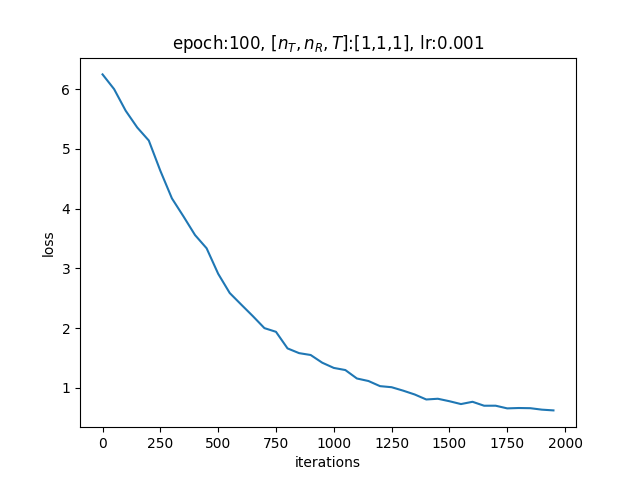
\includegraphics[width=0.7\textwidth]{Figure_1.png}
    \caption{hidden layer sizes: [64,32], $\mu_H=5, \sigma_H=0.2, \mu_W=0, \sigma_W=0.1 $}
\end{figure}


\end{frame}

%%%%%%%%%%%%%%%%%%%%%%%%%%%%%%%%%%%%%%%%%%%%%%%%%%%%%%%%%%%%%%%%%%
\begin{frame}{Simulation Result}
%%%%%%%%%%%%%%%%%%%%%%%%%%%%%%%%%%%%%%%%%%%%%%%%%%%%%%%%%%%%%%%%%%

\begin{figure}
    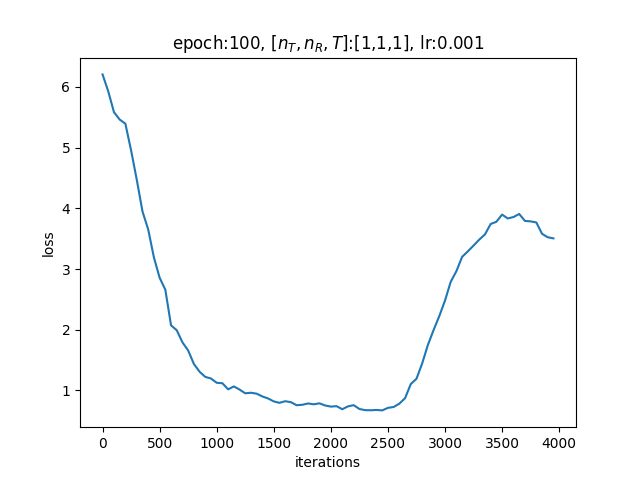
\includegraphics[width=0.7\textwidth]{Figure_2.png}
    \caption{increase the iterations from 2000 to 4000}
\end{figure}


\end{frame}


\end{document}
